\documentclass[a4paper, 10pt, dvipdfmx]{jlreq}

\usepackage{amsmath,amsfonts,amssymb}
\usepackage{bm}
\usepackage{mathtools}
\usepackage{siunitx}
\usepackage[dvipdfmx]{graphicx}
\usepackage[dvipdfmx]{color}
\usepackage[dvipdfmx, colorlinks=true, allcolors=blue]{hyperref}
\usepackage{listings, jlisting}
\usepackage{tikz}
\usepackage{physics}
\usepackage{url}

\Urlmuskip=0mu plus 10mu
\allowdisplaybreaks[4]
\frenchspacing
\definecolor{OliveGreen}{rgb}{0.0,0.6,0.0}
\definecolor{Orenge}{rgb}{0.89,0.55,0}
\definecolor{SkyBlue}{rgb}{0.28, 0.28, 0.95}
\lstset{
  language={c++},
  basicstyle={\ttfamily},
  identifierstyle={\small},
  ndkeywordstyle={\small},
  frame=single,
  breaklines=true,
  numbers=left,
  xrightmargin=0zw,
  xleftmargin=3zw,
  numberstyle={\scriptsize},
  lineskip=-0.9ex,
  keywordstyle={\small\bfseries\color{SkyBlue}},  
  commentstyle={\color{OliveGreen}}, 
  stringstyle={\small\ttfamily\color{Orenge}}    
}

\begin{document}

\title{2012年度 大問5}
\author{hari64boli64 (hari64boli64@gmail.com)}
\date{\today}
\maketitle

\section{問題}

\section{解答}

\subsection*{(1)}

\begin{align*}
  \det A=\begin{cases}
    2 & (N \text{ is odd})  \\
    0 & (N \text{ is even})
  \end{cases}
\end{align*}

\subsection*{(2)}

連結性より、$M \geq N - 1$ であることが必要。

rankの最大値は$N$なので、$M \leq N$であることが必要。

$M=N$のとき、サイクルか木$+1$本の辺であることが必要。

$M=N-1$のとき、木であることが必要。

これらは共に十分であることは、rankの定義から自明。

\subsection*{(3)}

奇数の時$1/2$

偶数の時$1010$か$0101$のような形になる。

\subsection*{(4)}

辺の重みとして正当なのは、$0,1/2,1$のいずれかのみ。

よって、サイクルと単独な辺の和集合となる。

\section{例}

\subsection*{(2)}

\begin{figure}[htbp]
  \begin{minipage}{0.33\hsize}
    \begin{center}
      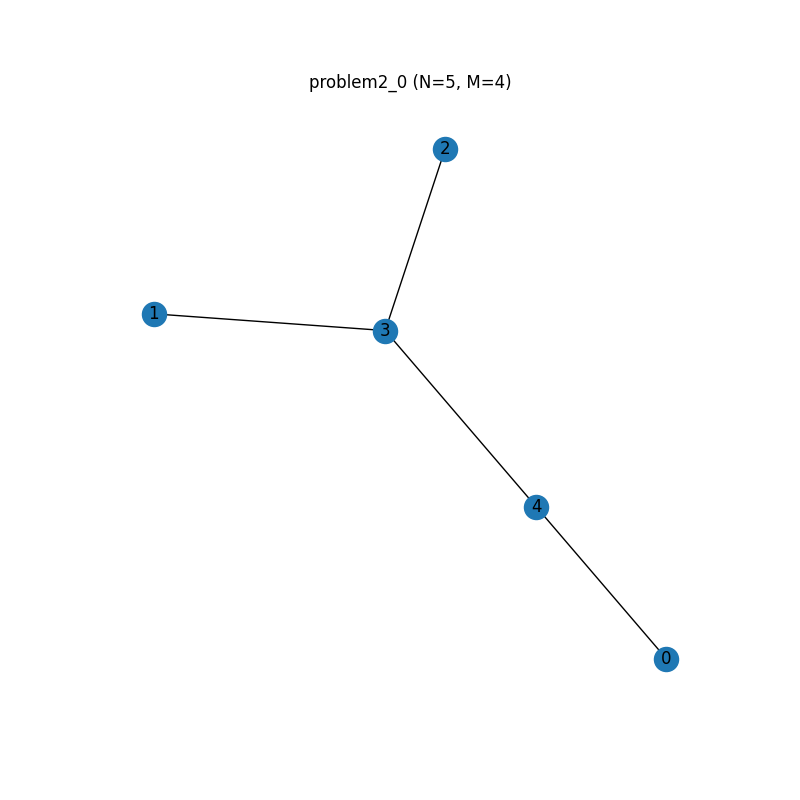
\includegraphics[width=40mm]{img_5/problem2_0.png}
    \end{center}
    \caption{2-0}
  \end{minipage}
  \begin{minipage}{0.33\hsize}
    \begin{center}
      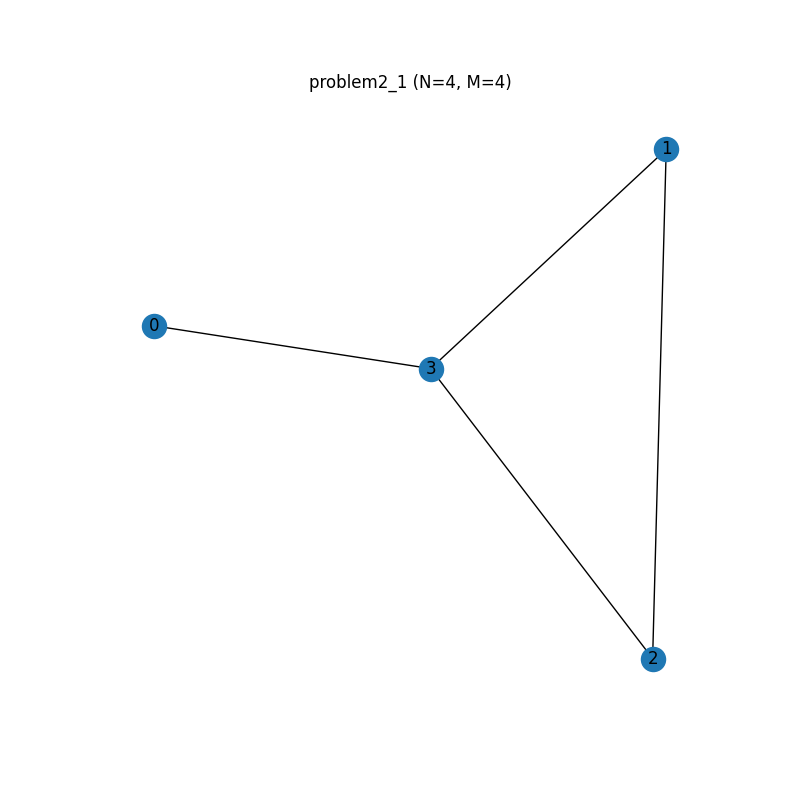
\includegraphics[width=40mm]{img_5/problem2_1.png}
    \end{center}
    \caption{2-1}
  \end{minipage}
  \begin{minipage}{0.33\hsize}
    \begin{center}
      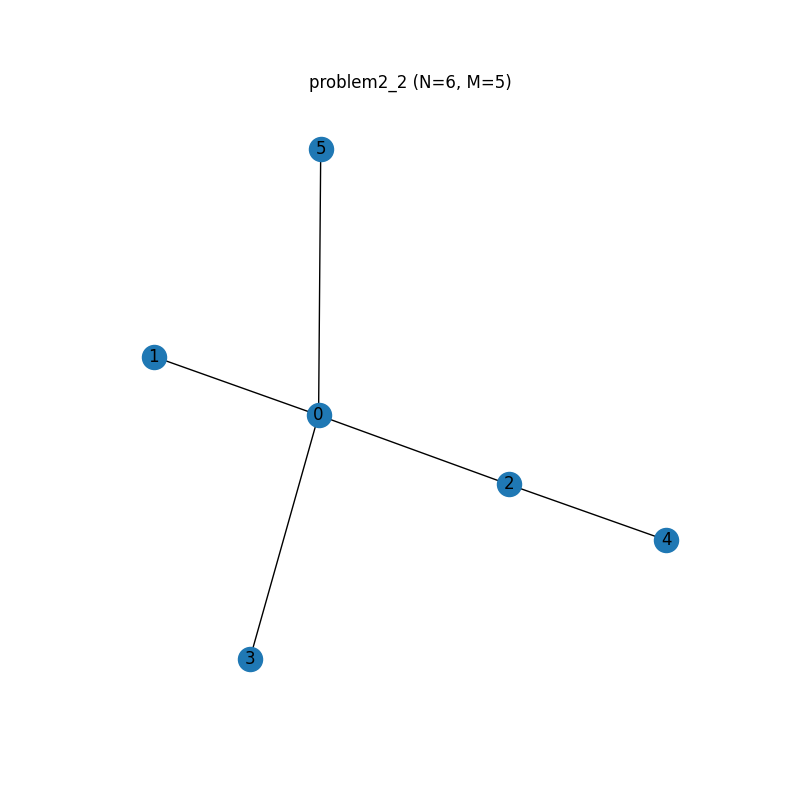
\includegraphics[width=40mm]{img_5/problem2_2.png}
    \end{center}
    \caption{2-2}
  \end{minipage}
\end{figure}


\begin{figure}[htbp]
  \begin{minipage}{0.33\hsize}
    \begin{center}
      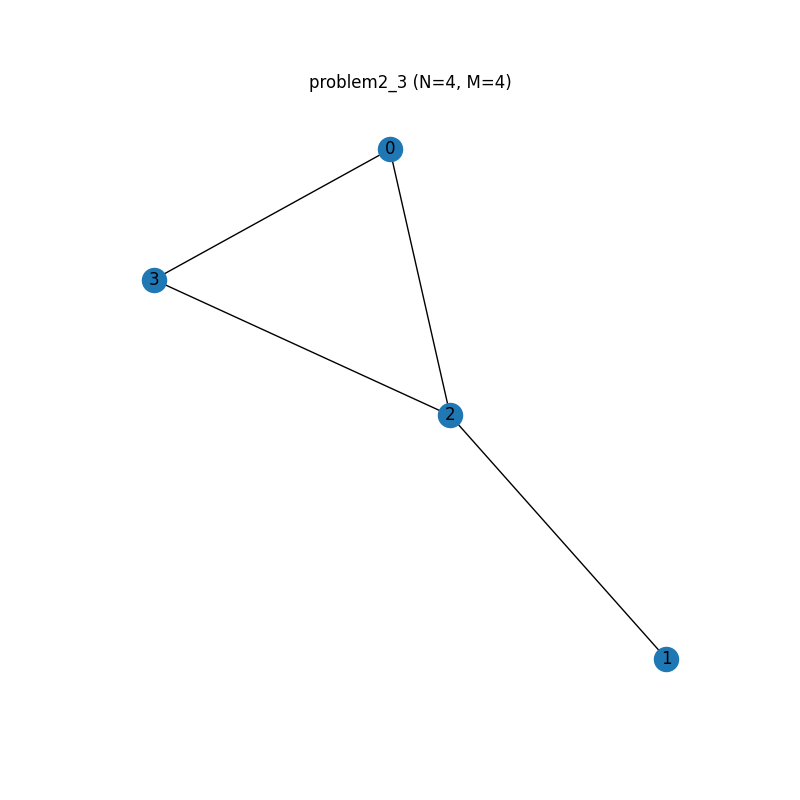
\includegraphics[width=40mm]{img_5/problem2_3.png}
    \end{center}
    \caption{2-3}
  \end{minipage}
  \begin{minipage}{0.33\hsize}
    \begin{center}
      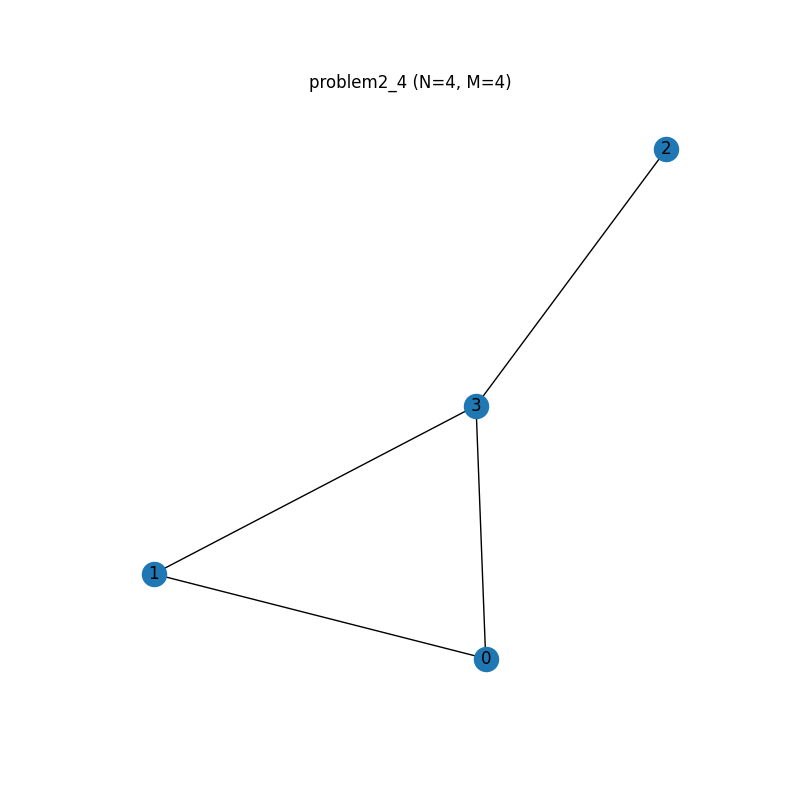
\includegraphics[width=40mm]{img_5/problem2_4.png}
    \end{center}
    \caption{2-4}
  \end{minipage}
  \begin{minipage}{0.33\hsize}
    \begin{center}
      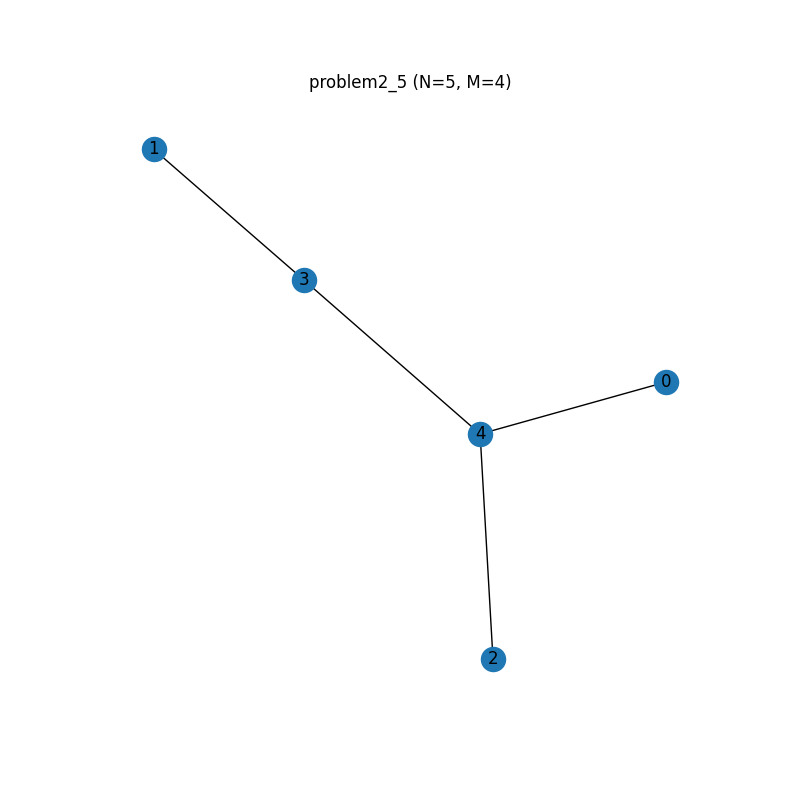
\includegraphics[width=40mm]{img_5/problem2_5.png}
    \end{center}
    \caption{2-5}
  \end{minipage}
\end{figure}

\begin{figure}[htbp]
  \begin{minipage}{0.33\hsize}
    \begin{center}
      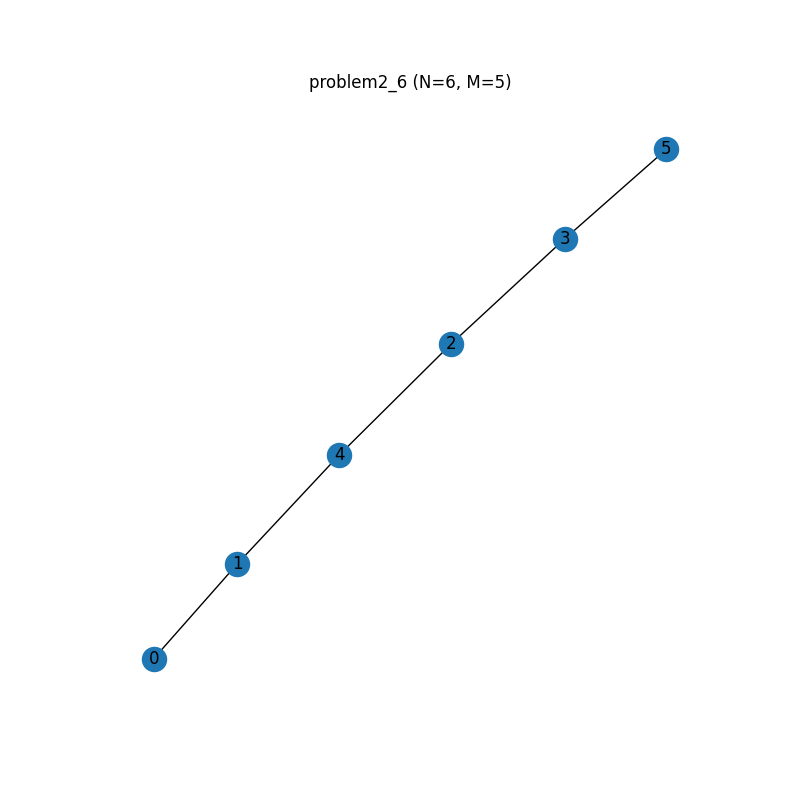
\includegraphics[width=40mm]{img_5/problem2_6.png}
    \end{center}
    \caption{2-6}
  \end{minipage}
  \begin{minipage}{0.33\hsize}
    \begin{center}
      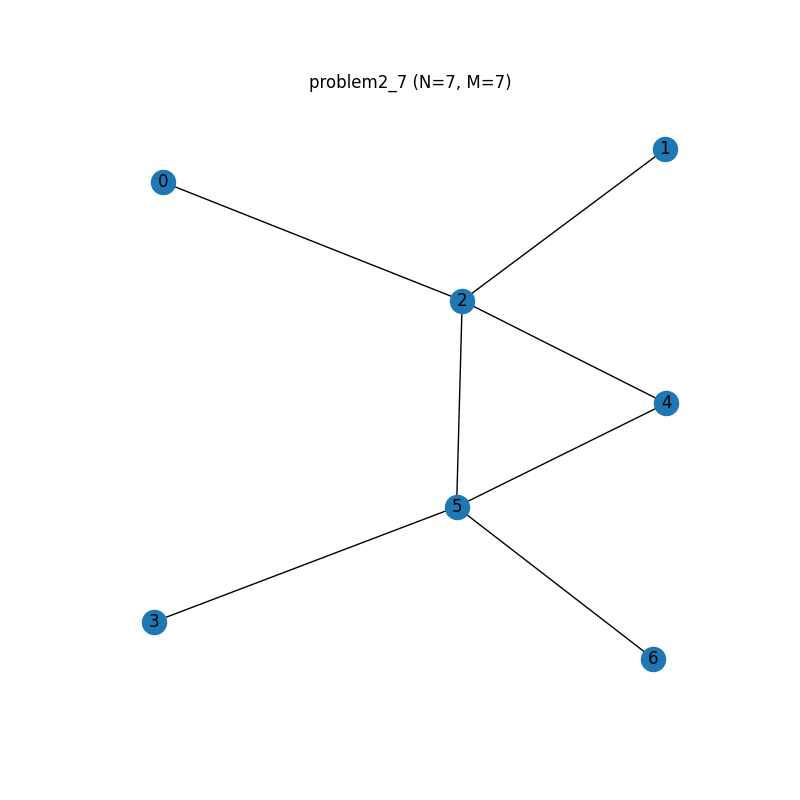
\includegraphics[width=40mm]{img_5/problem2_7.png}
    \end{center}
    \caption{2-7}
  \end{minipage}
  \begin{minipage}{0.33\hsize}
    \begin{center}
      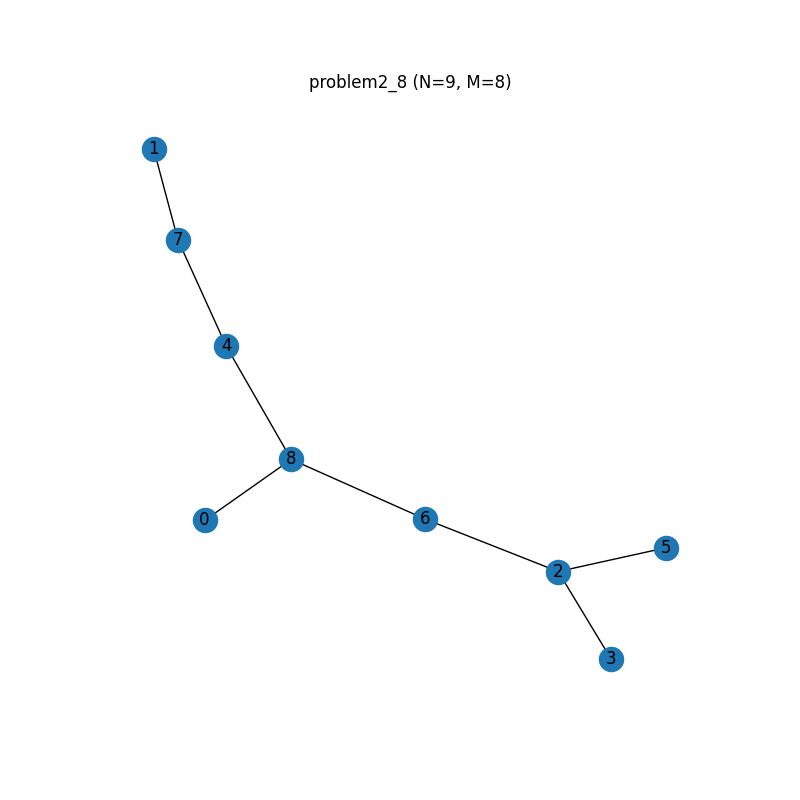
\includegraphics[width=40mm]{img_5/problem2_8.png}
    \end{center}
    \caption{2-8}
  \end{minipage}
\end{figure}

\begin{figure}[htbp]
  \begin{minipage}{0.33\hsize}
    \begin{center}
      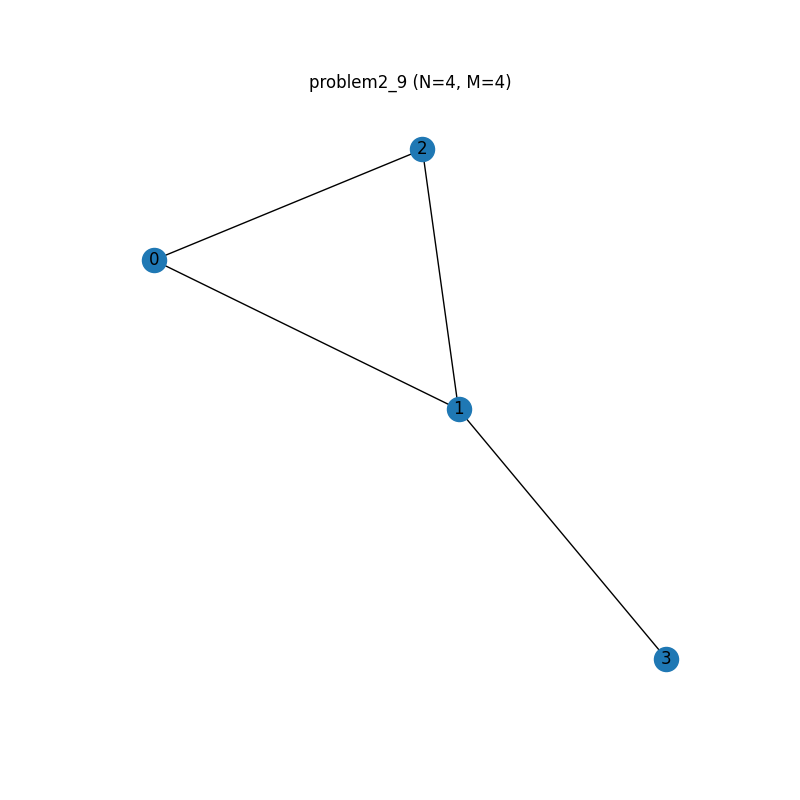
\includegraphics[width=40mm]{img_5/problem2_9.png}
    \end{center}
    \caption{2-9}
  \end{minipage}
  \begin{minipage}{0.33\hsize}
    \begin{center}
      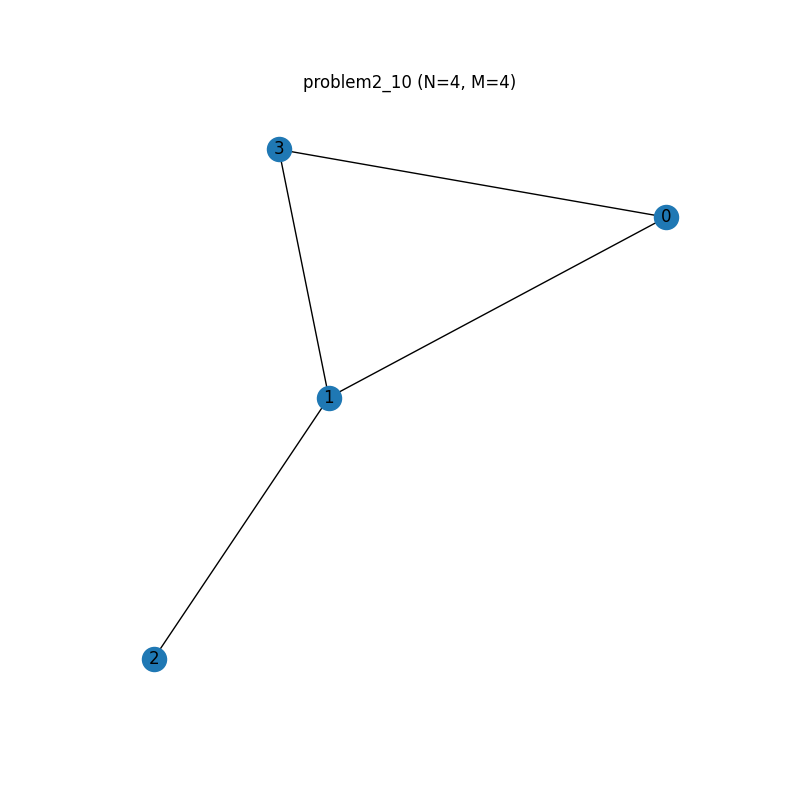
\includegraphics[width=40mm]{img_5/problem2_10.png}
    \end{center}
    \caption{2-10}
  \end{minipage}
  \begin{minipage}{0.33\hsize}
    \begin{center}
      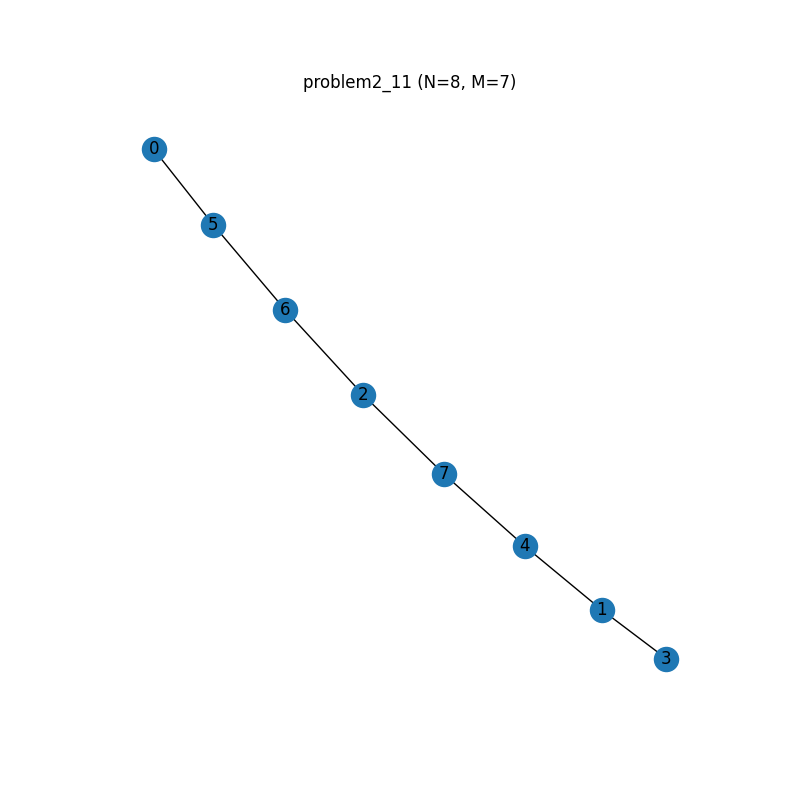
\includegraphics[width=40mm]{img_5/problem2_11.png}
    \end{center}
    \caption{2-11}
  \end{minipage}
\end{figure}

\begin{figure}[htbp]
  \begin{minipage}{0.33\hsize}
    \begin{center}
      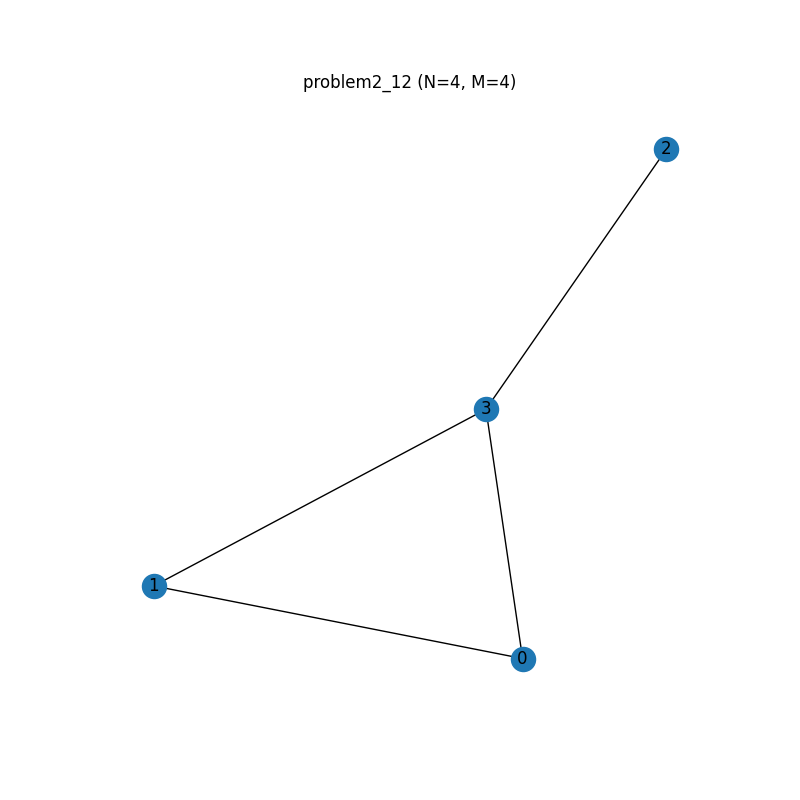
\includegraphics[width=40mm]{img_5/problem2_12.png}
    \end{center}
    \caption{2-12}
  \end{minipage}
  \begin{minipage}{0.33\hsize}
    \begin{center}
      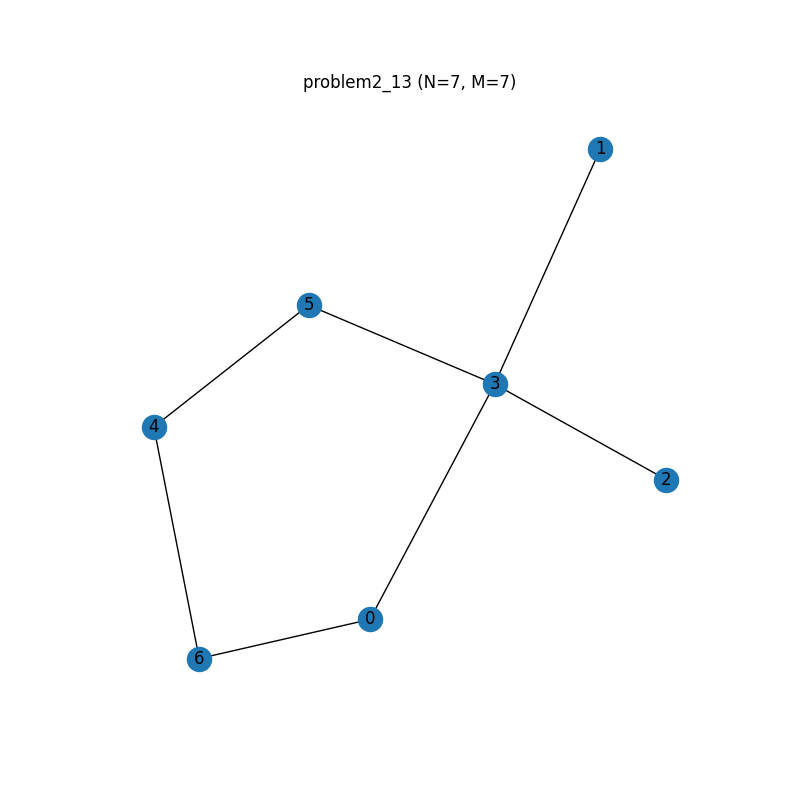
\includegraphics[width=40mm]{img_5/problem2_13.png}
    \end{center}
    \caption{2-13}
  \end{minipage}
  \begin{minipage}{0.33\hsize}
    \begin{center}
      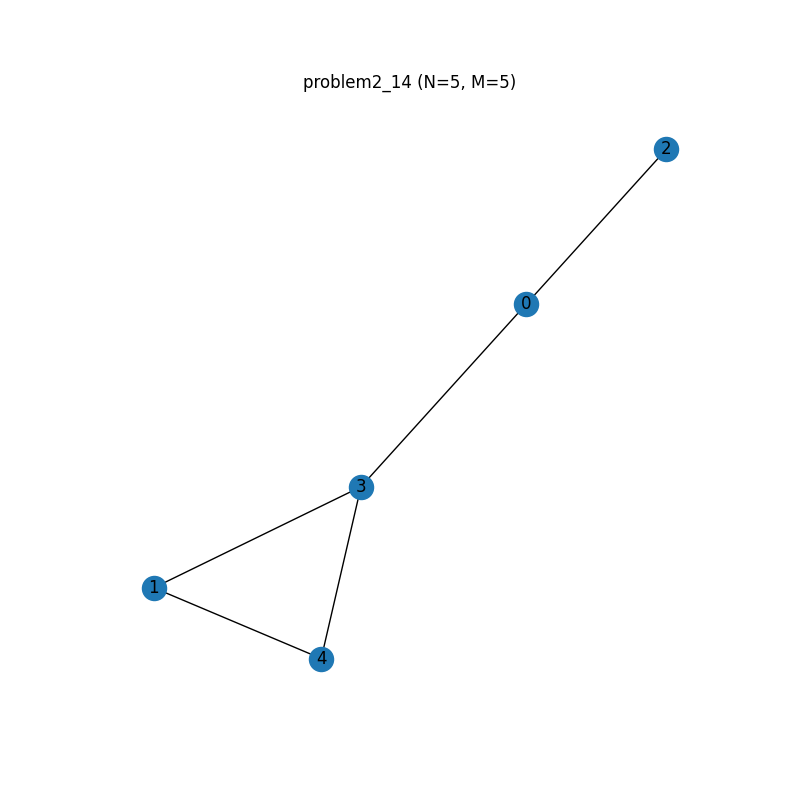
\includegraphics[width=40mm]{img_5/problem2_14.png}
    \end{center}
    \caption{2-14}
  \end{minipage}
\end{figure}

\subsection*{(4)}

以下の実行例は、辺の重みを$\{0,1/2,1\}$に限っている。なので、正当性の検証にはなっていない。
あくまで、そのような制限下での解を列挙したものである。

\begin{figure}[htbp]
  \begin{center}
    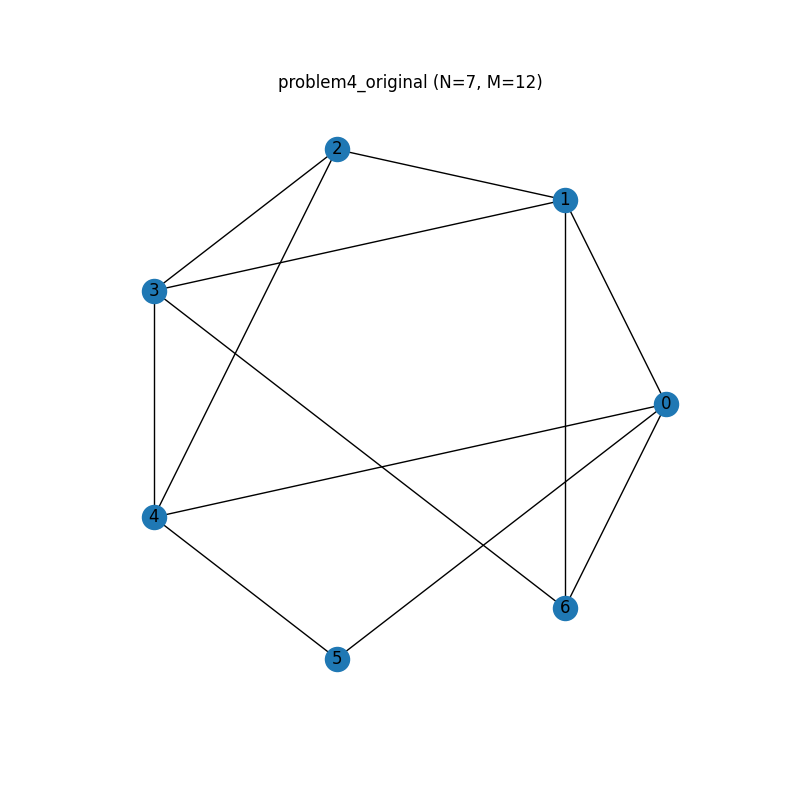
\includegraphics[height=80mm]{./img_5/problem4_original.png}
    \caption{original}
  \end{center}
\end{figure}

\begin{figure}[htbp]
  \begin{minipage}{0.33\hsize}
    \begin{center}
      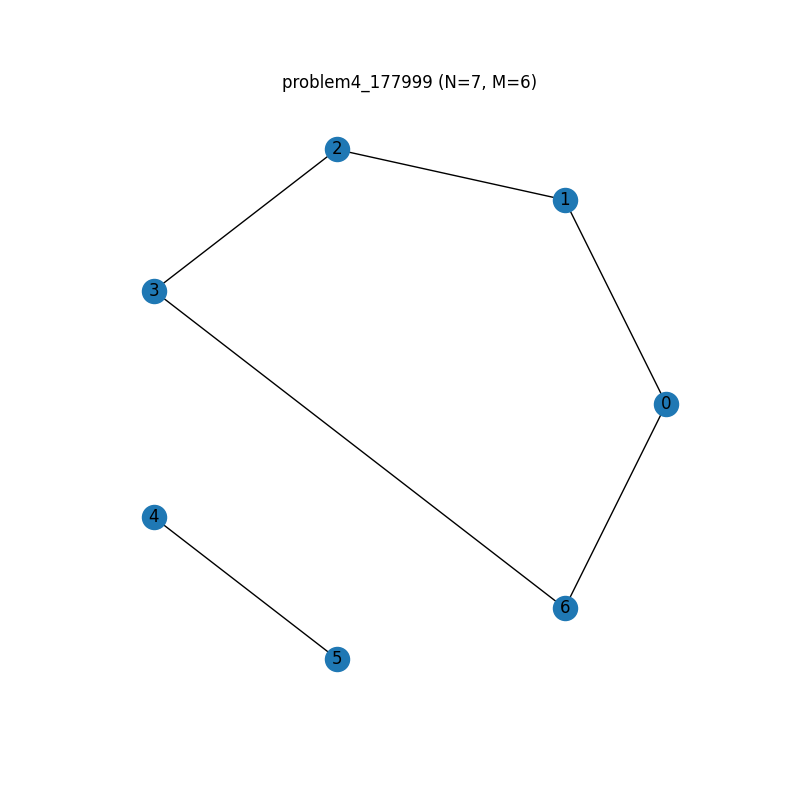
\includegraphics[width=40mm]{./img_5/problem4_177999.png}
    \end{center}
    \caption{id=177999}
  \end{minipage}
  \begin{minipage}{0.33\hsize}
    \begin{center}
      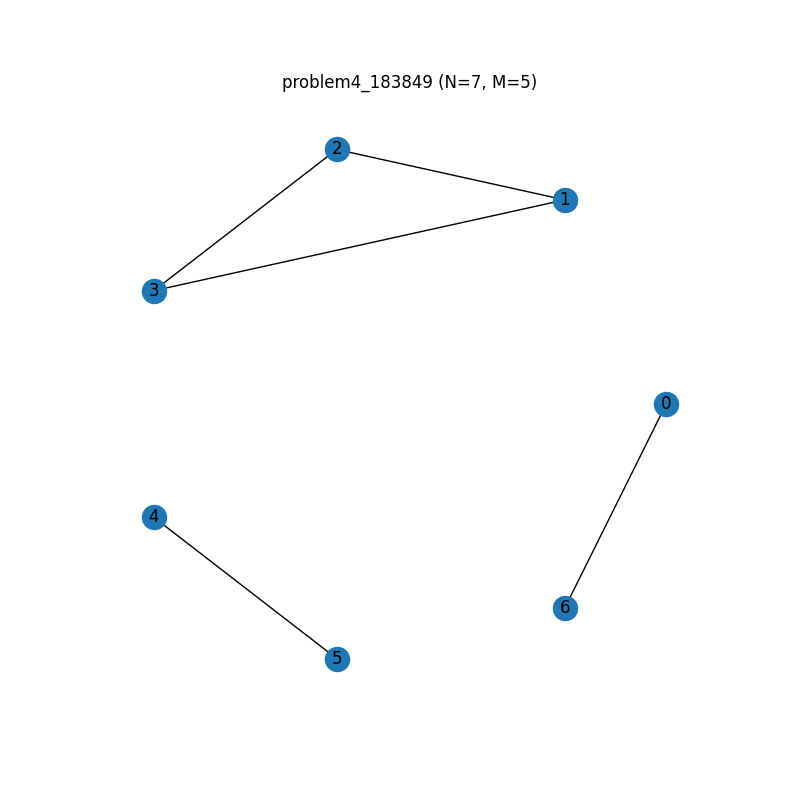
\includegraphics[width=40mm]{./img_5/problem4_183849.png}
    \end{center}
    \caption{id=183849}
  \end{minipage}
  \begin{minipage}{0.33\hsize}
    \begin{center}
      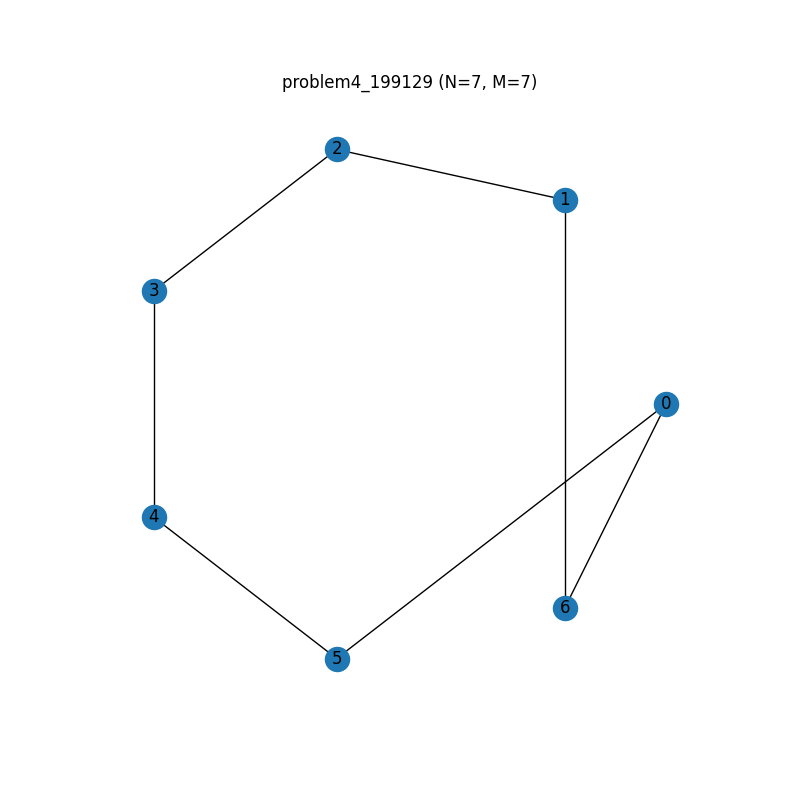
\includegraphics[width=40mm]{./img_5/problem4_199129.png}
    \end{center}
    \caption{id=199129}
  \end{minipage}
\end{figure}

\begin{figure}[htbp]
  \begin{minipage}{0.33\hsize}
    \begin{center}
      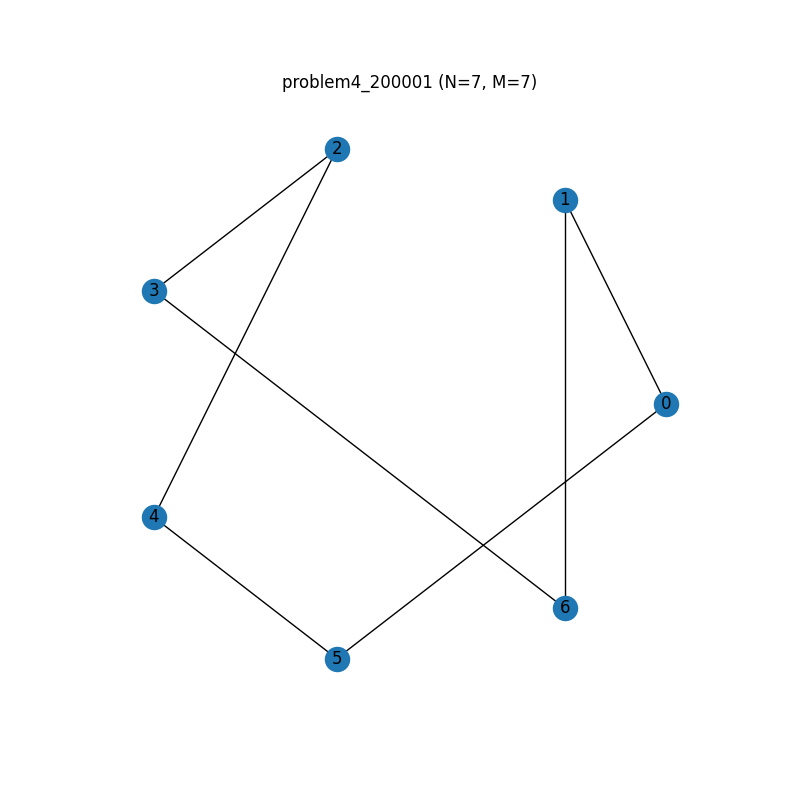
\includegraphics[width=40mm]{./img_5/problem4_200001.png}
    \end{center}
    \caption{id=200001}
  \end{minipage}
  \begin{minipage}{0.33\hsize}
    \begin{center}
      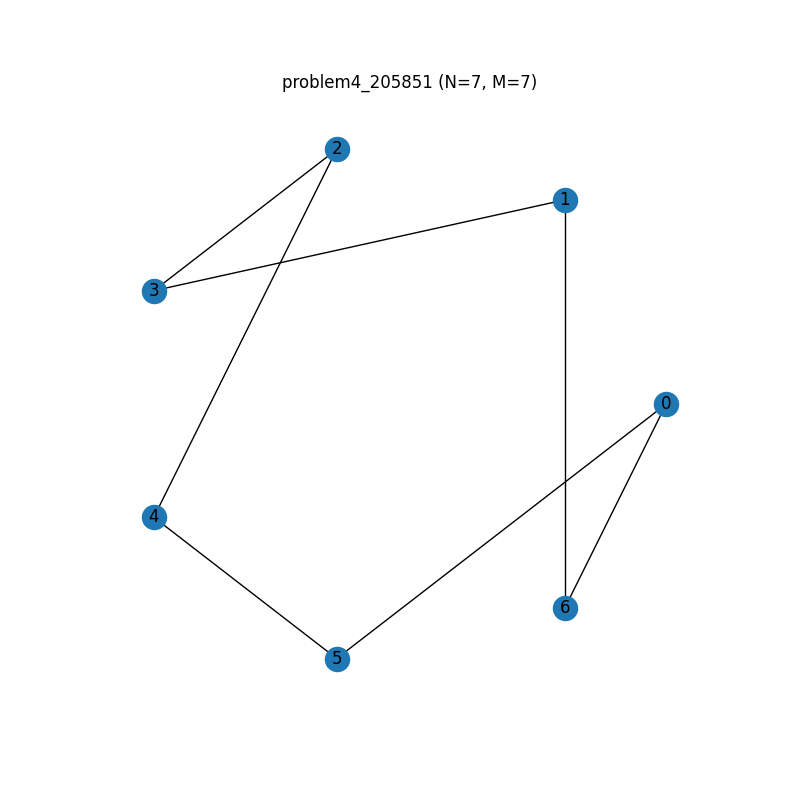
\includegraphics[width=40mm]{./img_5/problem4_205851.png}
    \end{center}
    \caption{id=205851}
  \end{minipage}
  \begin{minipage}{0.33\hsize}
    \begin{center}
      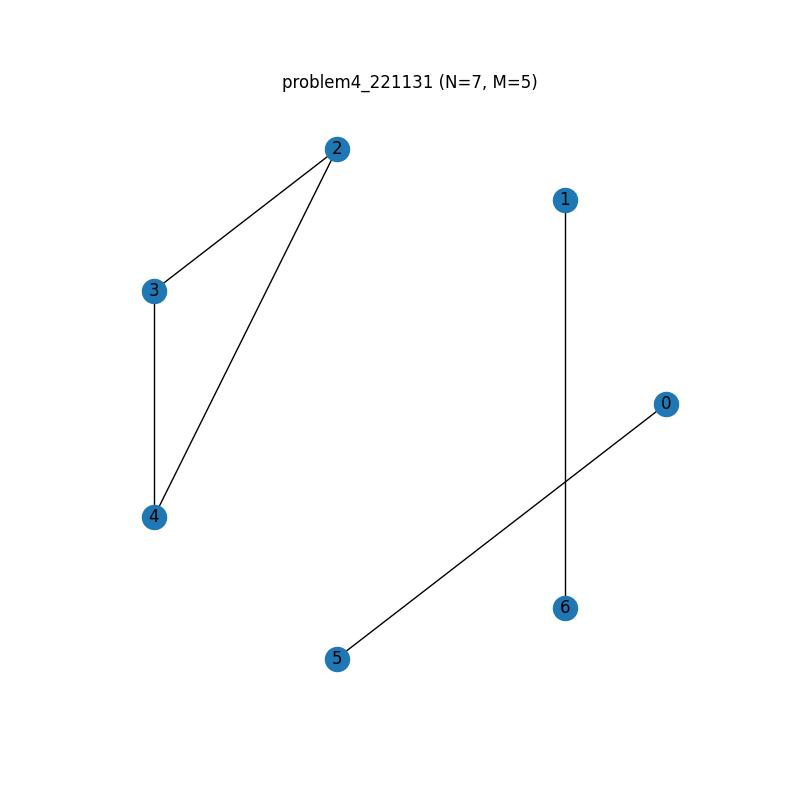
\includegraphics[width=40mm]{./img_5/problem4_221131.png}
    \end{center}
    \caption{id=221131}
  \end{minipage}
\end{figure}

\begin{figure}[htbp]
  \begin{minipage}{0.33\hsize}
    \begin{center}
      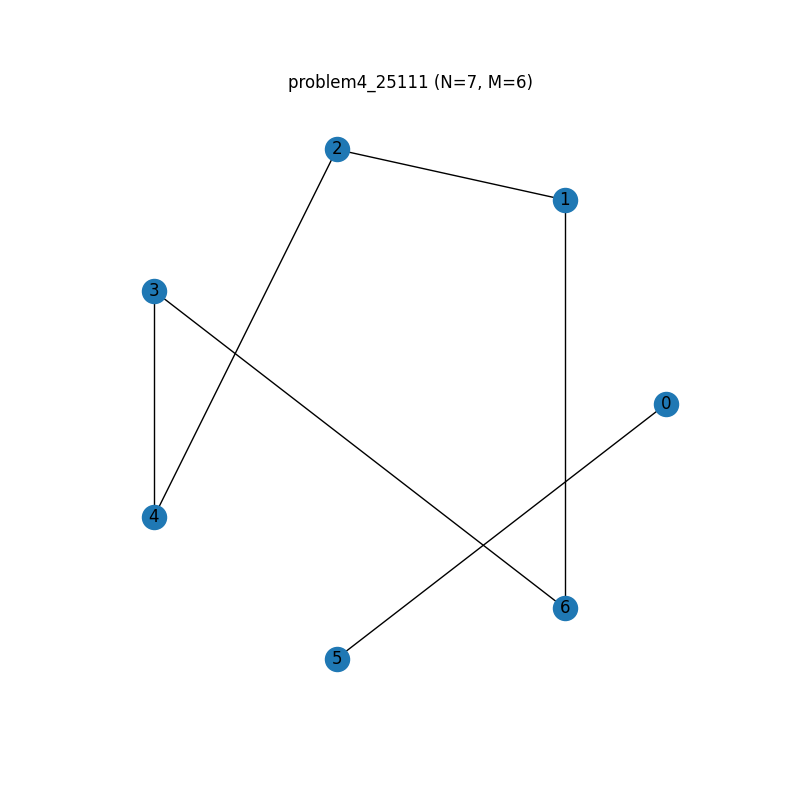
\includegraphics[width=40mm]{./img_5/problem4_25111.png}
    \end{center}
    \caption{id=25111}
  \end{minipage}
  \begin{minipage}{0.33\hsize}
    \begin{center}
      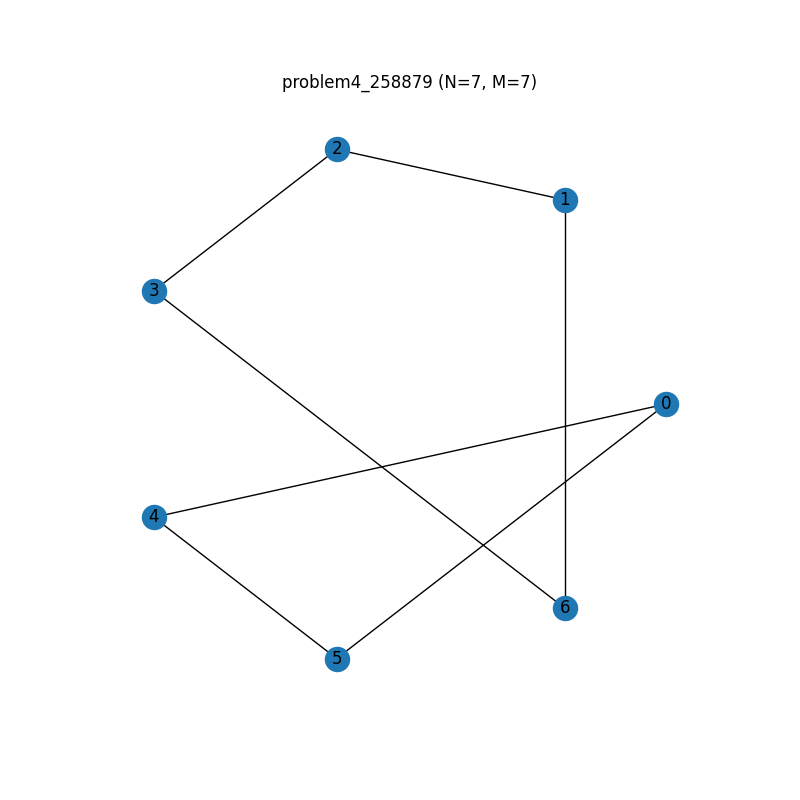
\includegraphics[width=40mm]{./img_5/problem4_258879.png}
    \end{center}
    \caption{id=258879}
  \end{minipage}
  \begin{minipage}{0.33\hsize}
    \begin{center}
      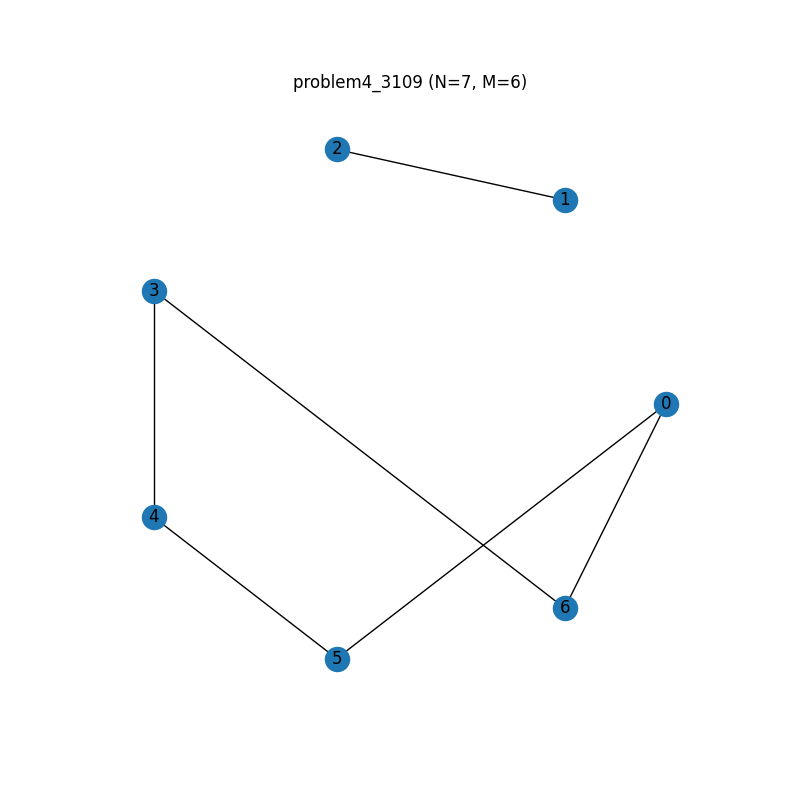
\includegraphics[width=40mm]{./img_5/problem4_3109.png}
    \end{center}
    \caption{id=3109}
  \end{minipage}
\end{figure}

\begin{figure}[htbp]
  \begin{minipage}{0.33\hsize}
    \begin{center}
      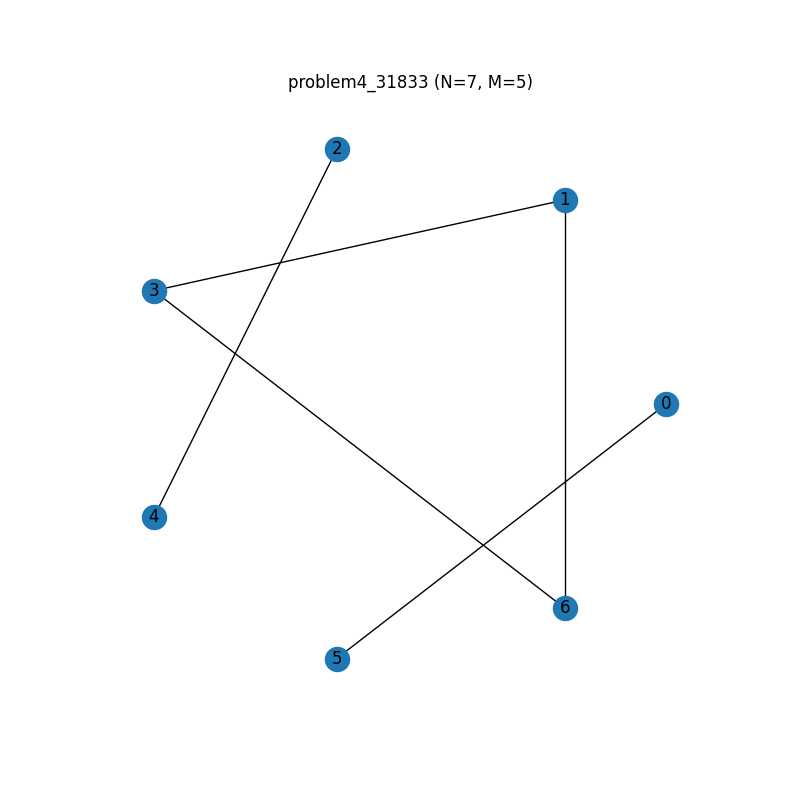
\includegraphics[width=40mm]{./img_5/problem4_31833.png}
    \end{center}
    \caption{id=31833}
  \end{minipage}
  \begin{minipage}{0.33\hsize}
    \begin{center}
      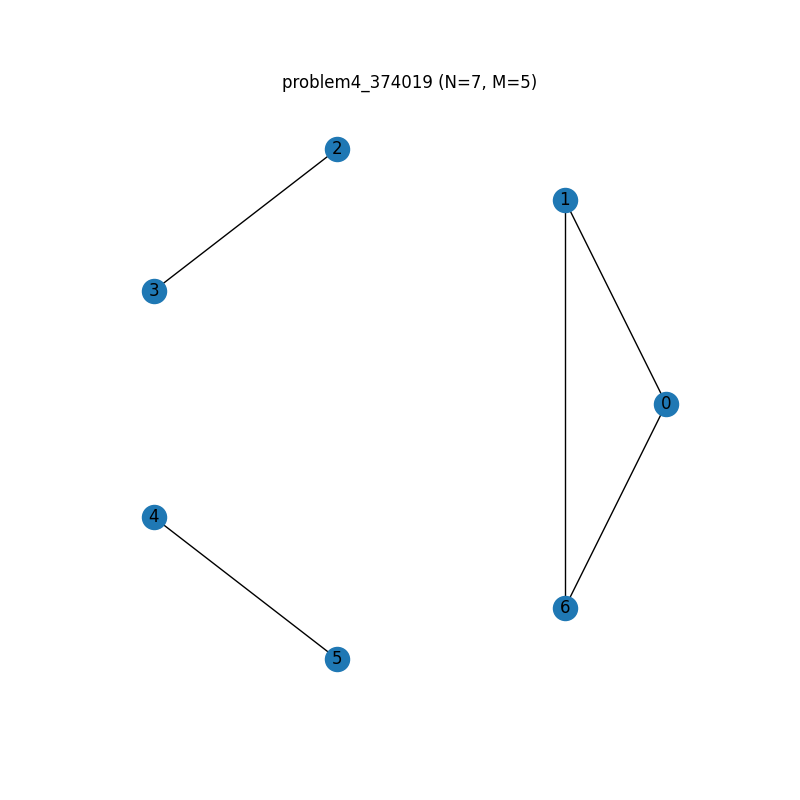
\includegraphics[width=40mm]{./img_5/problem4_374019.png}
    \end{center}
    \caption{id=374019}
  \end{minipage}
  \begin{minipage}{0.33\hsize}
    \begin{center}
      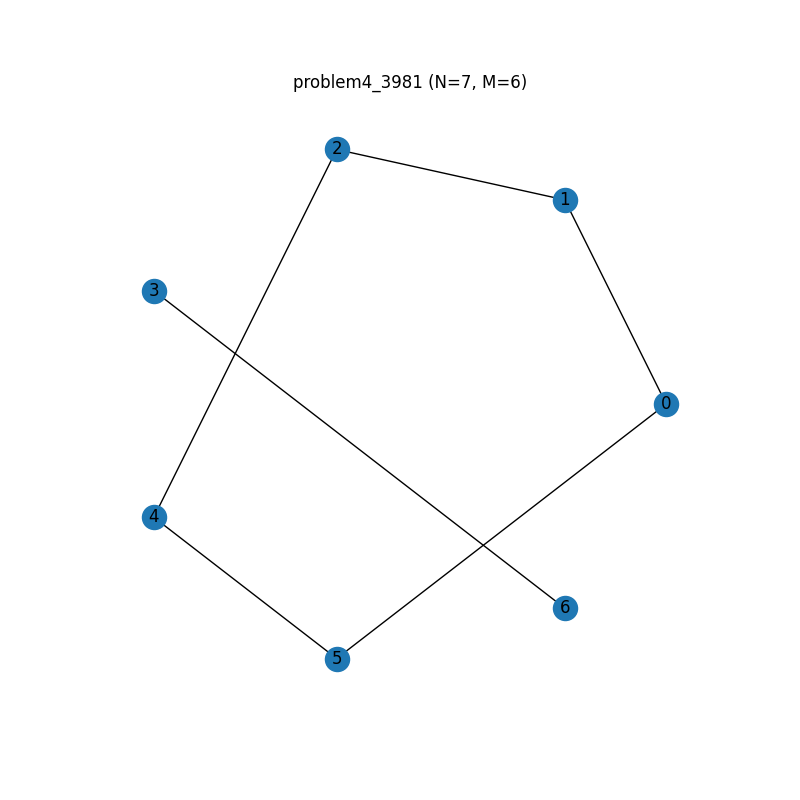
\includegraphics[width=40mm]{./img_5/problem4_3981.png}
    \end{center}
    \caption{id=3981}
  \end{minipage}
\end{figure}

\begin{figure}[htbp]
  \begin{minipage}{0.33\hsize}
    \begin{center}
      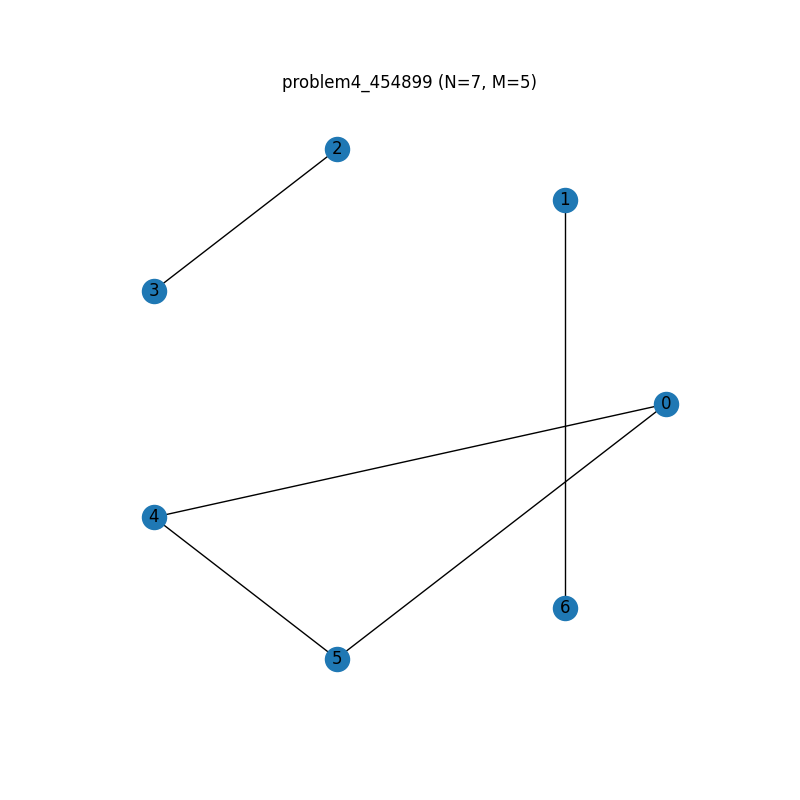
\includegraphics[width=40mm]{./img_5/problem4_454899.png}
    \end{center}
    \caption{id=454899}
  \end{minipage}
  \begin{minipage}{0.33\hsize}
    \begin{center}
      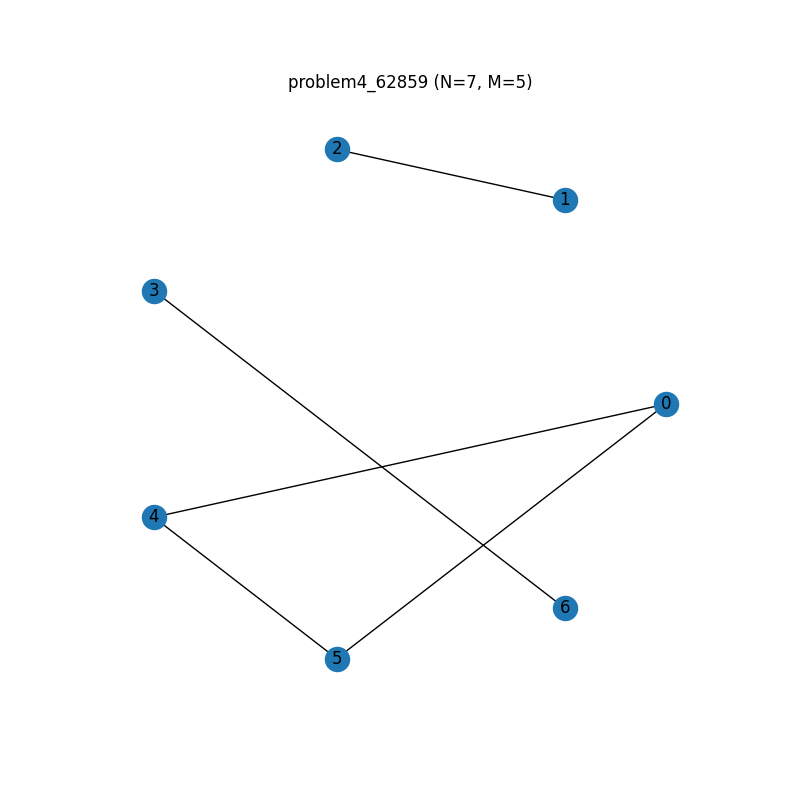
\includegraphics[width=40mm]{./img_5/problem4_62859.png}
    \end{center}
    \caption{id=62859}
  \end{minipage}
  \begin{minipage}{0.33\hsize}
    \begin{center}
      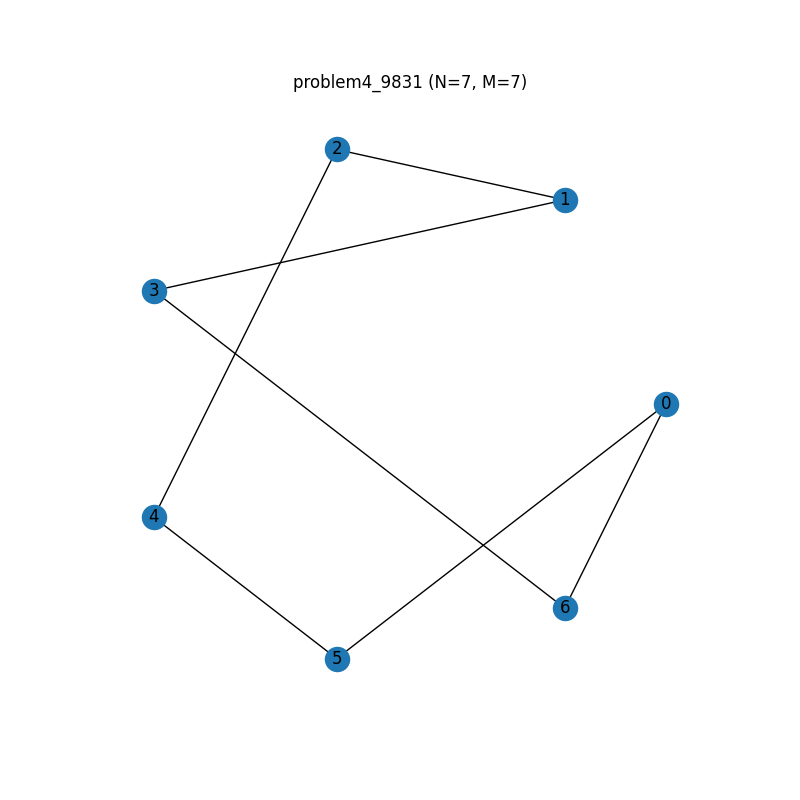
\includegraphics[width=40mm]{./img_5/problem4_9831.png}
    \end{center}
    \caption{id=9831}
  \end{minipage}
\end{figure}

\newpage

\section{おまけ}

\lstinputlisting[caption=vis,label=code:vis,language=Python]{5.py}

\end{document}
